\subsection{HTTP Live Streaming}
\label{sec:hls}

\begin{figure}[t]
  \centering
  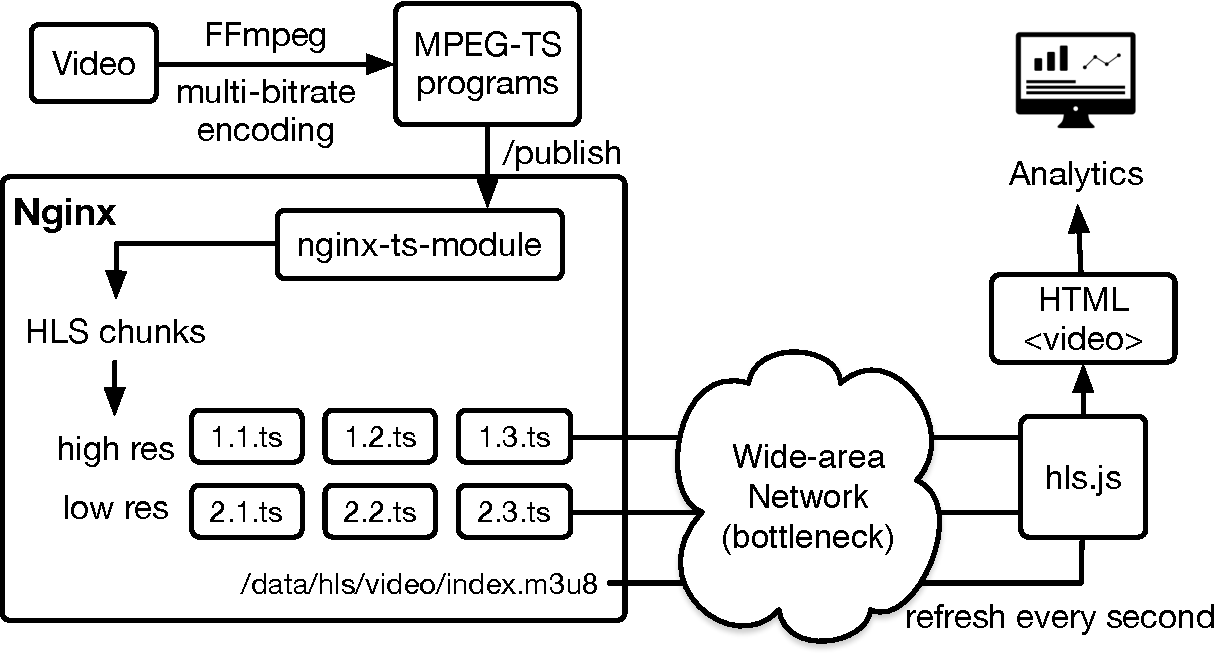
\includegraphics[width=\textwidth]{figures/hls.pdf}
  \caption{HLS setup. (Left) High-level overview: machine 1 generates a video
    and stores it in the server; machine 2 fetches the data and performs
    analytics. (Right) Detailed view: (1)~FFmpeg encodes video with multiple
    bitrates and groups them into MPEG-TS programs; (2)~\texttt{nginx-ts-module}
    then generates HLS chunks on the fly and stores them for nginx serving;
    (3)~the client (using \texttt{hls.js}) periodically fetches the latest index
    file (\texttt{index.m3u8}) and then downloads the right chunk according to
    network conditions.}
  \label{fig:hls-arch}
\end{figure}

HTTP Live Streaming (HLS)~\cite{pantos2016http} represents a class of HTTP-based
media streaming protocols. Other protocols include Adobe HTTP Dynamic
Streaming~\cite{adobestreaming}, Microsoft Smooth
Streaming~\cite{zambelli2009iis}, and a newer vendor-independent standard
DASH~\cite{michalos2012dynamic, sodagar2011mpeg}. These adaptive streaming
protocols are widely adopted for both video-on-demand (VoD) and live streaming
(such as Periscope).

Our setup (\autoref{fig:hls-arch}) resembles the setup of popular live streaming
services~\cite{wang2016anatomy}. We first describe each component of our
setup. We then discuss why these protocols are a poor match for wide-area
streaming analytics, despite their adaptation capability.

\para{Video.} We use \texttt{FFmpeg} to encode the video with multiple bitrates:
all levels use 30FPS, but different resolutions and H.264 encoding quality. Our
experiment uses six different bitrates---900p, 720p, 540p, 360p, all with normal
encoding quality; and 720p, 540p, with low encoding quality. To simulate live
video streaming, we then use \texttt{FFmpeg} to re-publish the stream to an
Nginx web server that accepts MPEG-TS (MPEG transport stream).

\para{Server.} Our web server is a nginx server compiled with plugin
\texttt{nginx-ts-module}~\cite{nginx-ts-module} that receives MPEG-TS over HTTP,
produces live HLS and DASH chunks. It creates an index file \texttt{index.m3u8}
that describes the media stream. During live streaming, the file is updated
whenever new chunks arrive. And the client needs to fetch the newest version of
\texttt{index.m3u8} to find out about new chunks. Typical streaming servers set
each chunk to be 2-10 seconds~\cite{mao2017neural, sun2016cs2p,
  wang2016anatomy}. For our low latency streaming, we configured the chunk
segment to be 1 second.

\para{Analytics.} The HTTP client reads the index file and then fetches each
chunk based on available bandwidth. Our client uses \texttt{hls.js}
\cite{hls.js}, a JavaScript library that implements an HLS client. It directly
plays the video inside an HTML5 video element. To avoid invoking the graphical
front-end of a browser, we use Puppeteer~\cite{puppeteer}, a NodeJS library that
provides a high-level API to control headless Chrome. During the runtime
experiment, instead of playing the video, we record the metadata with each
received chunk: its size, timestamp, and the quality level. We perform an
offline analysis of the log files to calculate the throughput, latency, and
accuracy.

Notice that the client-server relationship is reversed in HLS and \awstream{}. In
HLS, the server hosts video source files; the client fetches videos and
plays/computes. In \awstream{}, the client generates videos and pushes frames to
the server; the server performs video analytics.

\vspace{0.5em}

\para{Why HLS/DASH is a poor match for video analytics?} It is hard to achieve
ultra low latency using HLS/DASH. (1) HLS/DASH is pull-based. The client keeps
requesting for new chunks; (2) HLS/DASH uses chunking: shorter chunks enable a
lower latency, but induce a larger number of requests, and the chunk has to be
made ready before the client can start fetching. There are proposals to reduce
the latency, such as server push~\cite{wei2014low}, but they are still work in
progress. For some applications, the accuracy can also be poor if these videos
are limited to tuning resolution and encoding quality only, as demonstrated in
our PD evaluation.

%%% Local Variables:
%%% mode: latex
%%% TeX-master: "../network"
%%% End:
